\subsection{Validazione e collaudo}
\subsubsection{I Periodo}
\subsubsubsection{Prospetto orario}
La seguente tabella rappresenta la distribuzione oraria per ogni componente del gruppo nel I periodo della fase di validazione e collaudo:
\begin{table}[H]
\begin{center}
\rowcolors{2}{gray!25}{white}
\renewcommand{\arraystretch}{1.25}
\begin{tabular}{ m{0.20\textwidth}<{\centering}  m{0.06\textwidth}<{\centering} m{0.06\textwidth}<{\centering} m{0.06\textwidth}<{\centering}  m{0.06\textwidth}<{\centering}  m{0.06\textwidth}<{\centering}  m{0.06\textwidth}<{\centering}  m{0.20\textwidth}<{\centering}   }
	\rowcolor{darkblue}
	\textcolor{white}{\textbf{Componente}} &\textcolor{white}{\textbf{Re}}&\textcolor{white}{\textbf{Pt}}&\textcolor{white}{\textbf{An}}&\textcolor{white}{\textbf{Am}}&\textcolor{white}{\textbf{Pr}}&\textcolor{white}{\textbf{Ve}}&\textcolor{white}{\textbf{Ore complessive}}\\ 
	Edoardo Pavan & 0 & 0 & 0 & 0 & 0 & 1 & 1 \\	
	
	Francesco Protopapa & 1 & 0 & 0 & 1 & 0 & 1 & 3 \\

	Greta Cavedon & 1 & 1 & 0 & 1 & 0 & 1 & 4 \\
	
	Luciano Wu & 0 & 5 & 0 & 0 & 0 & 0 &5 \\
	
	Matteo Basso & 0 & 2 & 0 & 1 & 0 & 1 & 4 \\
	
	Michele Gatto & 0 & 4 & 0 & 0 & 0 & 0 & 4 \\
	
	Pietro Villatora & 1 & 4 & 0 & 0 & 0 & 0 & 5 \\
	
	\textbf{Ore totali ruolo} & 3 & 16 & 0 & 3 & 0 & 4 & 26 \\

\end{tabular}
\caption{Distribuzione oraria per ogni componente nel I periodo della fase di verifica e collaudo}
\end{center}
\end{table}

La tabella può essere rappresentata anche in forma visiva dal seguente grafico:
\begin{figure}[H]
\centering
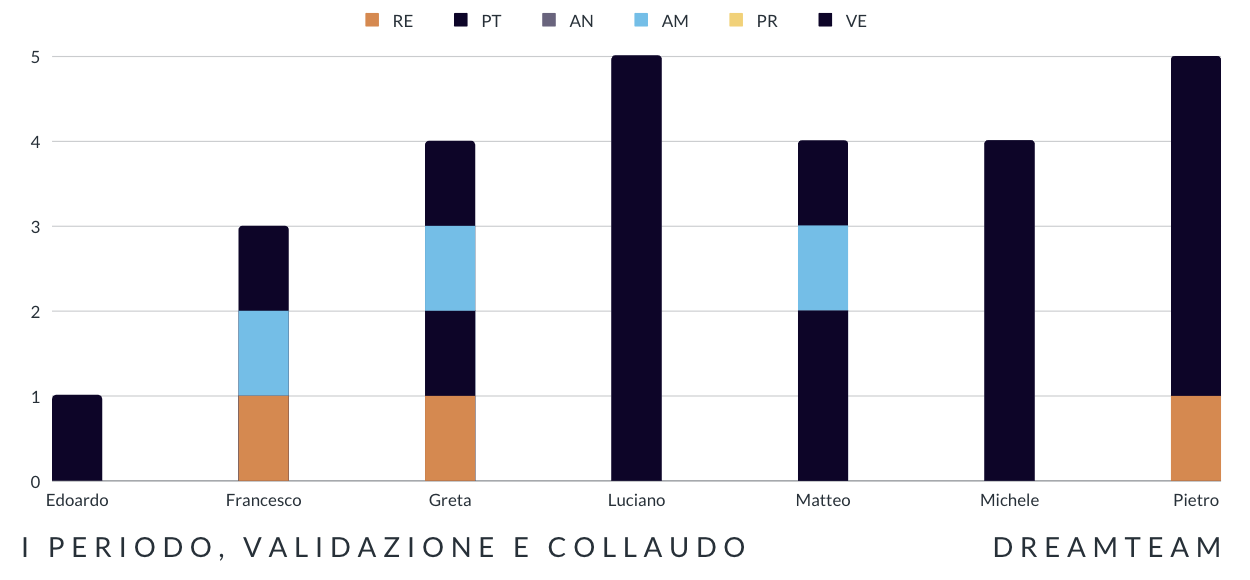
\includegraphics[scale=0.65]{Sezioni/SezioniPreventivo/grafici/Validazione_collaudo_I_periodo.png}
\caption{Istogramma della ripartizione delle ore nel I periodo della fase di validazione e collaudo}
\end{figure}

\subsubsubsection{Prospetto economico}
La seguente tabella rappresenta le ore totali dedicate ad ogni ruolo e il costo in euro:

\begin{table}[H]
\begin{center}
\rowcolors{2}{gray!25}{white}
\renewcommand{\arraystretch}{1.5}
\begin{tabular}{ m{0.3\textwidth}<{\centering}  m{0.2\textwidth}<{\centering} m{0.2\textwidth}<{\centering}}
	\rowcolor{darkblue}
	\textcolor{white}{\textbf{Ruolo}}&\textcolor{white}{\textbf{Totale ore}}&\textcolor{white}{\textbf{Costo totale (\euro)}}\\ 

	Responsabile  & 3 & 90 \\	
	
	Progettista & 16 & 400 \\
	
	Analista & 0 & 0 \\

	Amministratore & 3 & 60 \\
	
	Programmatore & 0 & 0 \\
	
	Verificatore & 4 & 60 \\
	
	\textbf{Totale} & 26 & 610 \\
	
\end{tabular}
\caption{Prospetto del costo per ruoli nel I periodo della fase di verifica e collaudo}
\end{center}
\end{table}

La tabella può essere rappresentata anche in forma visiva dal seguente aerogramma:
\begin{figure}[H]
\centering
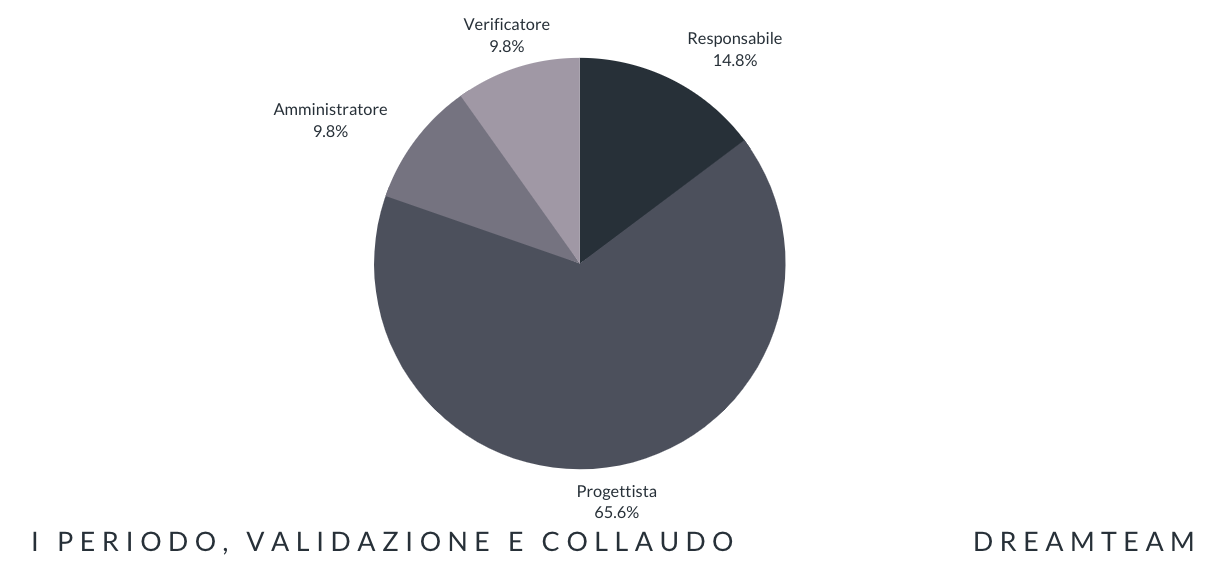
\includegraphics[scale=0.65]{Sezioni/SezioniPreventivo/grafici/Validazione_I_periodo_costi.png}
\caption{Grafico a torta della ripartizione per ruolo dei costi nel I periodo della fase di validazione e collaudo}
\end{figure}



\subsubsection{II Periodo}
\subsubsubsection{Prospetto orario}
La seguente tabella rappresenta la distribuzione oraria per ogni componente del gruppo nel II periodo della fase di verifica e collaudo:
\begin{table}[H]
\begin{center}
\rowcolors{2}{gray!25}{white}
\renewcommand{\arraystretch}{1.25}
\begin{tabular}{ m{0.20\textwidth}<{\centering}  m{0.06\textwidth}<{\centering} m{0.06\textwidth}<{\centering} m{0.06\textwidth}<{\centering}  m{0.06\textwidth}<{\centering}  m{0.06\textwidth}<{\centering}  m{0.06\textwidth}<{\centering}  m{0.20\textwidth}<{\centering}   }
	\rowcolor{darkblue}
	\textcolor{white}{\textbf{Componente}} &\textcolor{white}{\textbf{Re}}&\textcolor{white}{\textbf{Pt}}&\textcolor{white}{\textbf{An}}&\textcolor{white}{\textbf{Am}}&\textcolor{white}{\textbf{Pr}}&\textcolor{white}{\textbf{Ve}}&\textcolor{white}{\textbf{Ore complessive}}\\ 
	Edoardo Pavan & 2 & 0 & 0 & 0 & 9 & 2 & 13 \\	
	
	Francesco Protopapa & 1 & 0 & 0 & 2 & 8 & 3 & 14 \\

	Greta Cavedon & 1 & 0 & 0 & 1 & 6 & 5 & 13 \\
	
	Luciano Wu & 0 & 1 & 0 & 0 & 9 & 2 & 12 \\
	
	Matteo Basso & 0 & 0 & 0 & 2 & 4 & 2 & 8 \\
	
	Michele Gatto & 1 & 0 & 0 & 0 & 6 & 2 & 9 \\
	
	Pietro Villatora & 1 & 0 & 0 & 0 & 6 & 2 & 9 \\
	
	\textbf{Ore totali ruolo} & 6 & 1 & 0 & 5 & 48 & 18 & 78 \\

\end{tabular}
\caption{Distribuzione oraria per ogni componente nel II periodo della fase di verifica e collaudo}
\end{center}
\end{table}

La tabella può essere rappresentata anche in forma visiva dal seguente grafico:
\begin{figure}[H]
\centering
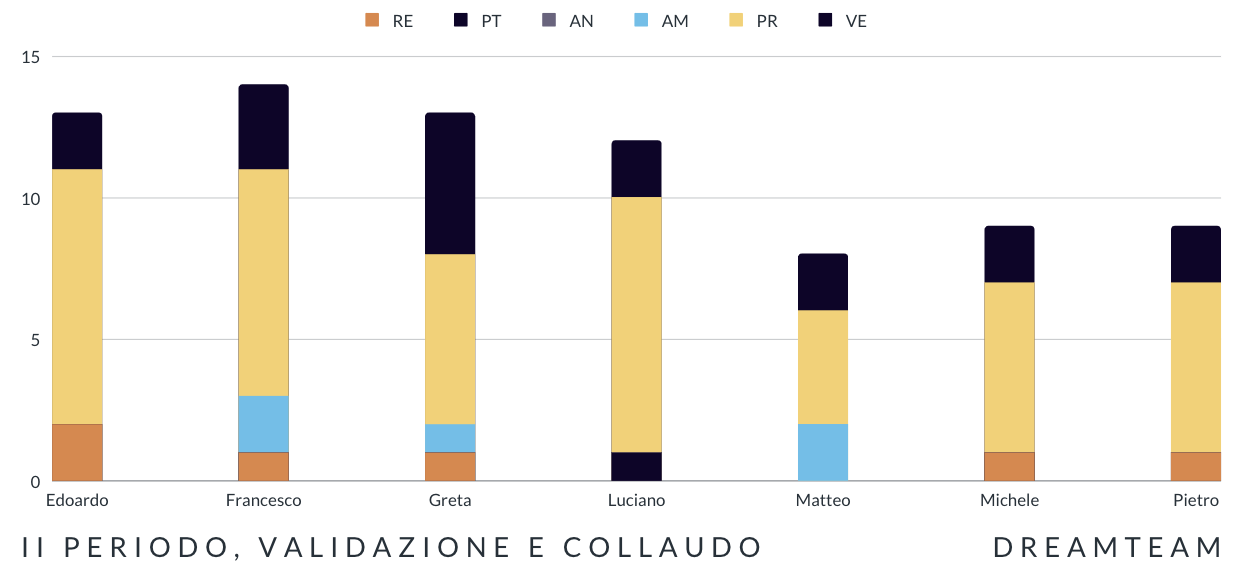
\includegraphics[scale=0.65]{Sezioni/SezioniPreventivo/grafici/Validazione_collaudo_II_periodo.png}
\caption{Istogramma della ripartizione delle ore nel II periodo della fase di validazione e collaudo}
\end{figure}

\subsubsubsection{Prospetto economico}
La seguente tabella rappresenta le ore totali dedicate ad ogni ruolo e il costo in euro:

\begin{table}[H]
\begin{center}
\rowcolors{2}{gray!25}{white}
\renewcommand{\arraystretch}{1.5}
\begin{tabular}{ m{0.3\textwidth}<{\centering}  m{0.2\textwidth}<{\centering} m{0.2\textwidth}<{\centering}}
	\rowcolor{darkblue}
	\textcolor{white}{\textbf{Ruolo}}&\textcolor{white}{\textbf{Totale ore}}&\textcolor{white}{\textbf{Costo totale (\euro)}}\\ 

	Responsabile  & 6 & 180 \\	
	
	Progettista & 1 & 25 \\
	
	Analista & 0 & 0 \\

	Amministratore & 5 & 100 \\
	
	Programmatore & 48 & 720 \\
	
	Verificatore & 18 & 270 \\
	
	\textbf{Totale} & 78 & 1295 \\
	
\end{tabular}
\caption{Prospetto del costo per ruoli nel II periodo della fase di verifica e collaudo}
\end{center}
\end{table}

La tabella può essere rappresentata anche in forma visiva dal seguente aerogramma:
\begin{figure}[H]
\centering
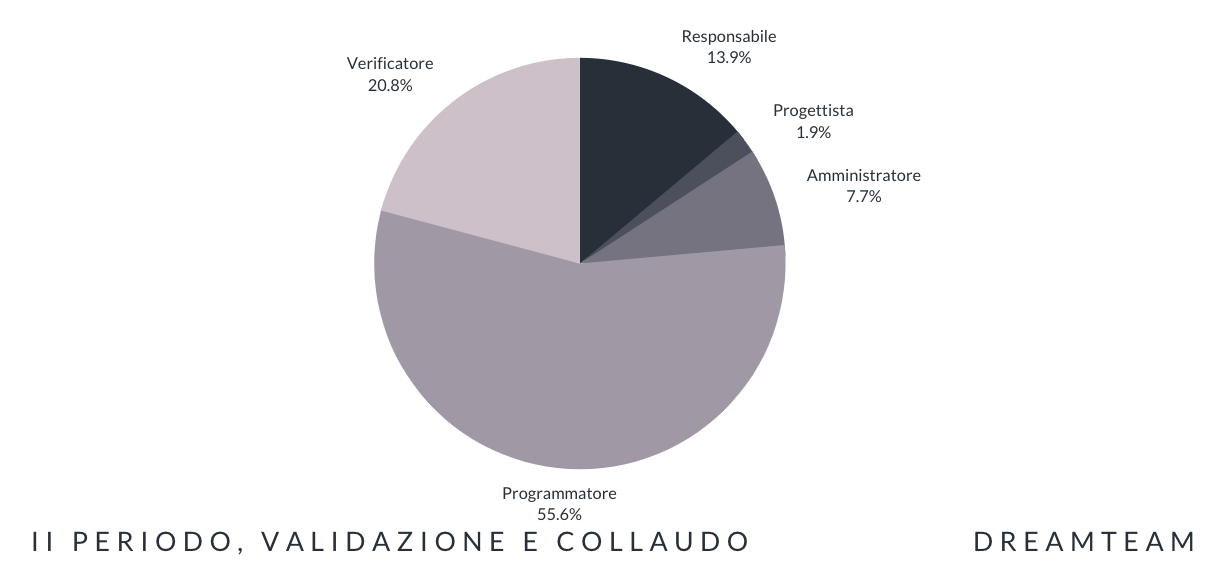
\includegraphics[scale=0.65]{Sezioni/SezioniPreventivo/grafici/Validazione_II_periodo_costi.png}
\caption{Grafico a torta della ripartizione per ruolo dei costi nel II periodo della fase di validazione e collaudo}
\end{figure}



\subsubsection{III Periodo}
\subsubsubsection{Prospetto orario}
La seguente tabella rappresenta la distribuzione oraria per ogni componente del gruppo nel III periodo della fase di verifica e collaudo:
\begin{table}[H]
\begin{center}
\rowcolors{2}{gray!25}{white}
\renewcommand{\arraystretch}{1.25}
\begin{tabular}{ m{0.20\textwidth}<{\centering}  m{0.06\textwidth}<{\centering} m{0.06\textwidth}<{\centering} m{0.06\textwidth}<{\centering}  m{0.06\textwidth}<{\centering}  m{0.06\textwidth}<{\centering}  m{0.06\textwidth}<{\centering}  m{0.20\textwidth}<{\centering}   }
	\rowcolor{darkblue}
	\textcolor{white}{\textbf{Componente}} &\textcolor{white}{\textbf{Re}}&\textcolor{white}{\textbf{Pt}}&\textcolor{white}{\textbf{An}}&\textcolor{white}{\textbf{Am}}&\textcolor{white}{\textbf{Pr}}&\textcolor{white}{\textbf{Ve}}&\textcolor{white}{\textbf{Ore complessive}}\\ 
	Edoardo Pavan & 0 & 0 & 0 & 0 & 1 & 1 & 2 \\	
	
	Francesco Protopapa & 1 & 0 & 0 & 1 & 1 & 1 & 4 \\

	Greta Cavedon & 1 & 0 & 0 & 2 & 0 & 1 & 4 \\
	
	Luciano Wu & 0 & 1 & 0 & 0 & 1 & 1 & 3 \\
	
	Matteo Basso & 0 & 0 & 0 & 1 & 0 & 1 & 2 \\
	
	Michele Gatto & 2  & 1 & 0 & 0 & 0 & 1 & 4 \\
	
	Pietro Villatora & 1 & 1 & 0 & 0 & 1 & 0 & 3 \\
	
	\textbf{Ore totali ruolo} & 5 & 3 & 0 & 4 & 4 & 6 & 22 \\

\end{tabular}
\caption{Distribuzione oraria per ogni componente nel III periodo della fase di verifica e collaudo}
\end{center}
\end{table}

La tabella può essere rappresentata anche in forma visiva dal seguente grafico:
\begin{figure}[H]
\centering
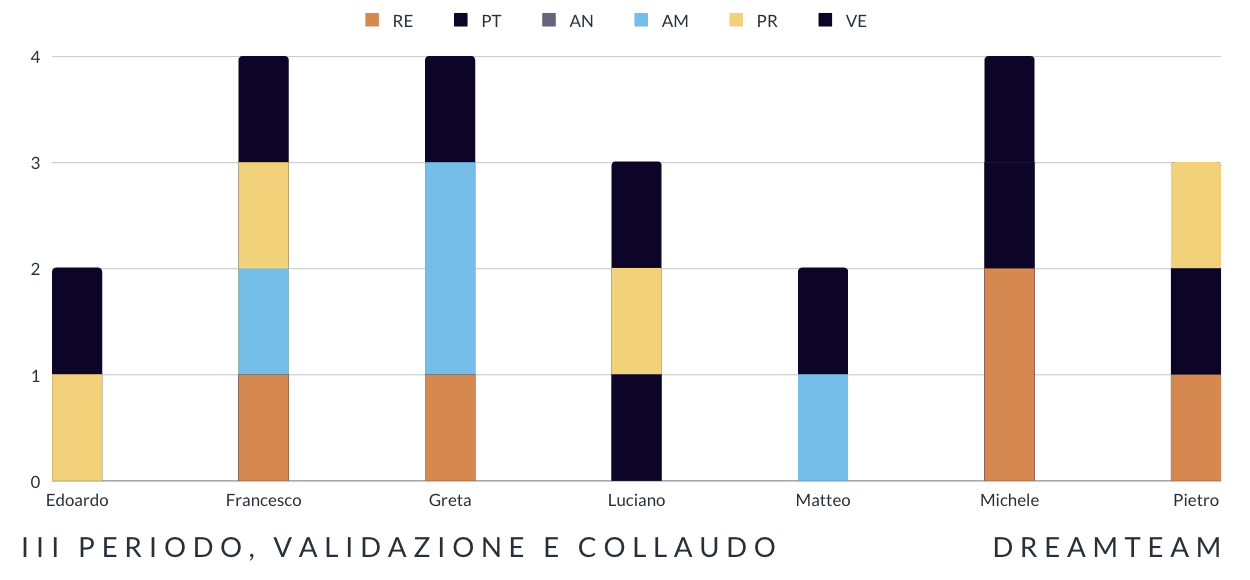
\includegraphics[scale=0.65]{Sezioni/SezioniPreventivo/grafici/Validazione_collaudo_III_periodo.png}
\caption{Istogramma della ripartizione delle ore nel III periodo della fase di validazione e collaudo}
\end{figure}

\subsubsubsection{Prospetto economico}
La seguente tabella rappresenta le ore totali dedicate ad ogni ruolo e il costo in euro:

\begin{table}[H]
\begin{center}
\rowcolors{2}{gray!25}{white}
\renewcommand{\arraystretch}{1.5}
\begin{tabular}{ m{0.3\textwidth}<{\centering}  m{0.2\textwidth}<{\centering} m{0.2\textwidth}<{\centering}}
	\rowcolor{darkblue}
	\textcolor{white}{\textbf{Ruolo}}&\textcolor{white}{\textbf{Totale ore}}&\textcolor{white}{\textbf{Costo totale (\euro)}}\\ 

	Responsabile  & 5 & 150 \\	
	
	Progettista & 3 & 75 \\
	
	Analista & 0 & 0 \\

	Amministratore & 4 & 80 \\
	
	Programmatore & 4 & 60 \\
	
	Verificatore & 6 & 90 \\
	
	\textbf{Totale} & 22 & 455 \\
	
\end{tabular}
\caption{Prospetto del costo per ruoli nel III periodo della fase di verifica e collaudo}
\end{center}
\end{table}

La tabella può essere rappresentata anche in forma visiva dal seguente aerogramma:
\begin{figure}[H]
\centering
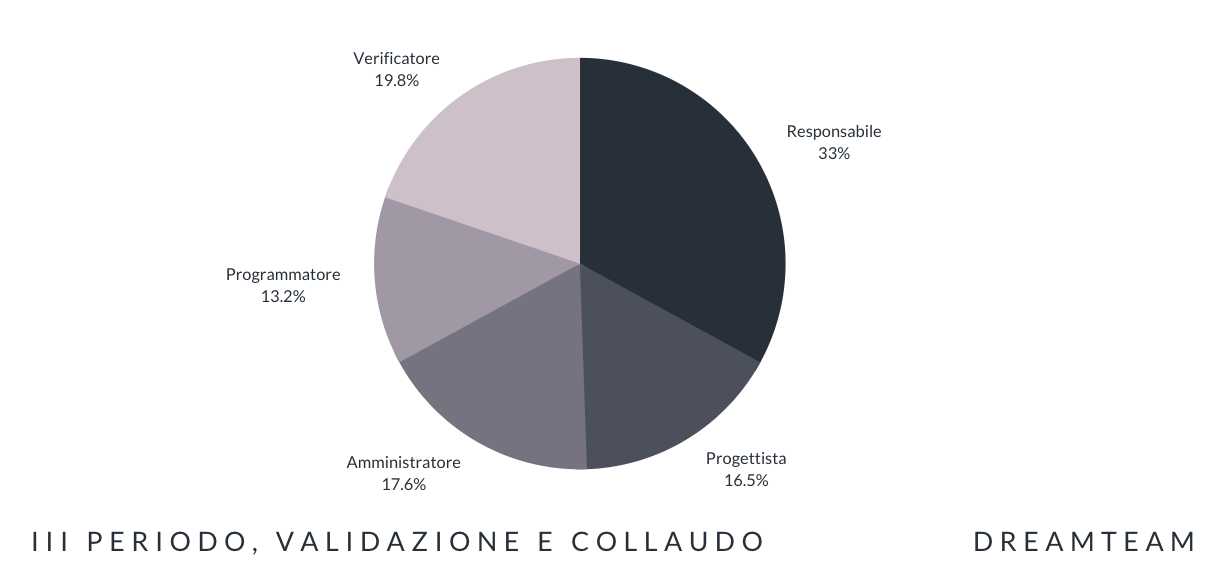
\includegraphics[scale=0.65]{Sezioni/SezioniPreventivo/grafici/Validazione_III_periodo_costi.png}
\caption{Grafico a torta della ripartizione per ruolo dei costi nel III periodo della fase di validazione e collaudo}
\end{figure}




\subsubsection{Fase complessiva}
\subsubsubsection{Prospetto orario}
La seguente tabella rappresenta la distribuzione oraria per ogni componente del gruppo nella fase di verifica e collaudo:
\begin{table}[H]
\begin{center}
\rowcolors{2}{gray!25}{white}
\renewcommand{\arraystretch}{1.25}
\begin{tabular}{ m{0.20\textwidth}<{\centering}  m{0.06\textwidth}<{\centering} m{0.06\textwidth}<{\centering} m{0.06\textwidth}<{\centering}  m{0.06\textwidth}<{\centering}  m{0.06\textwidth}<{\centering}  m{0.06\textwidth}<{\centering}  m{0.20\textwidth}<{\centering}   }
	\rowcolor{darkblue}
	\textcolor{white}{\textbf{Componente}} &\textcolor{white}{\textbf{Re}}&\textcolor{white}{\textbf{Pt}}&\textcolor{white}{\textbf{An}}&\textcolor{white}{\textbf{Am}}&\textcolor{white}{\textbf{Pr}}&\textcolor{white}{\textbf{Ve}}&\textcolor{white}{\textbf{Ore complessive}}\\ 
	Edoardo Pavan & 2 & 0 & 0 & 0 & 10 & 4 & 16 \\	
	
	Francesco Protopapa & 3 & 0 & 0 & 4 & 9 & 5 & 21 \\

	Greta Cavedon & 3 & 1 & 0 & 4 & 6 & 7 & 21 \\
	
	Luciano Wu & 0 & 7 & 0 & 0 & 10 & 3 & 20 \\
	
	Matteo Basso & 0 & 2 & 0 & 4 & 4 & 4 & 14 \\
	
	Michele Gatto & 3 & 5 & 0 & 0 & 6 & 3 & 17 \\
	
	Pietro Villatora & 3 & 5 & 0 & 0 & 7 & 2 & 17 \\
	
	\textbf{Ore totali ruolo} & 14 & 20 & 0 & 12 & 52 & 28 & 126\\

\end{tabular}
\caption{Distribuzione oraria per ogni componente nella fase di verifica e collaudo}
\end{center}
\end{table}

La tabella può essere rappresentata anche in forma visiva dal seguente grafico:
\begin{figure}[H]
\centering
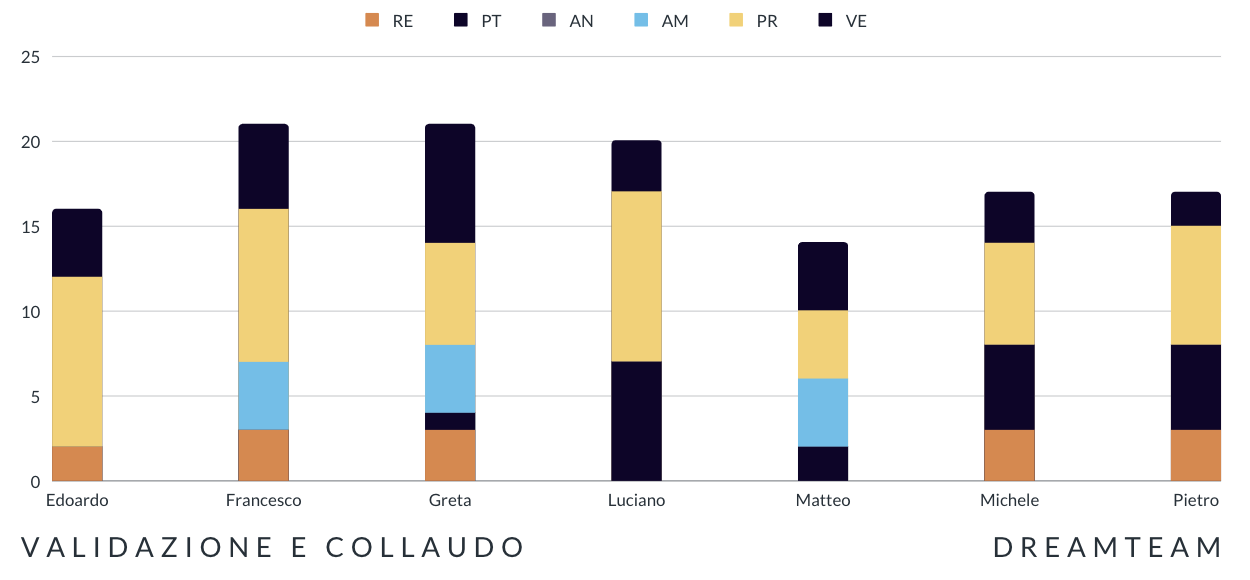
\includegraphics[scale=0.65]{Sezioni/SezioniPreventivo/grafici/Validazione_collaudo.png}
\caption{Istogramma della ripartizione delle ore  nella fase di validazione e collaudo}
\end{figure}

\subsubsubsection{Prospetto economico}
La seguente tabella rappresenta le ore totali dedicate ad ogni ruolo e il costo in euro:

\begin{table}[H]
\begin{center}
\rowcolors{2}{gray!25}{white}
\renewcommand{\arraystretch}{1.5}
\begin{tabular}{ m{0.3\textwidth}<{\centering}  m{0.2\textwidth}<{\centering} m{0.2\textwidth}<{\centering}}
	\rowcolor{darkblue}
	\textcolor{white}{\textbf{Ruolo}}&\textcolor{white}{\textbf{Totale ore}}&\textcolor{white}{\textbf{Costo totale (\euro)}}\\ 

	Responsabile  & 14 & 420 \\	
	
	Progettista & 20 & 500 \\
	
	Analista & 0 & 0 \\

	Amministratore & 12 & 240 \\
	
	Programmatore & 52 & 780 \\
	
	Verificatore & 28 & 420 \\
	
	\textbf{Totale} & 126 & 2360 \\
	
\end{tabular}
\caption{Prospetto del costo per ruoli nella fase di verifica e collaudo}
\end{center}
\end{table}

La tabella può essere rappresentata anche in forma visiva dal seguente aerogramma:
\begin{figure}[H]
\centering
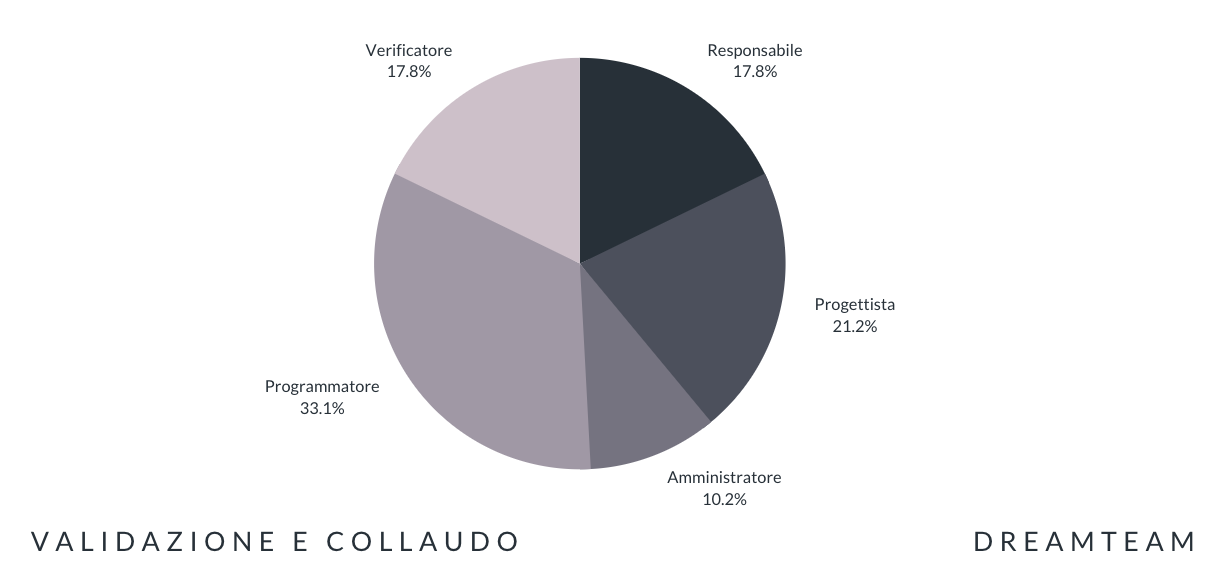
\includegraphics[scale=0.65]{Sezioni/SezioniPreventivo/grafici/Validazione_costi.png}
\caption{Grafico a torta della ripartizione per ruolo dei costi nella fase di validazione e collaudo}
\end{figure}
